%**************************************************************************
%* SpringSim 2017 Author Kit
%*
%* Word Processing System: TeXnicCenter and MiKTeX
%*
%**************************************************************************

\documentclass{scspaperproc}

\usepackage{latexsym}
\usepackage{graphicx}
\usepackage{mathptmx}
\usepackage{amsmath}
\usepackage{amsfonts}
\usepackage{amssymb}
\usepackage{amsbsy}
\usepackage{amsthm}
%% \usepackage{color}   % Needed to color text for drafts

%% \usepackage{algorithm}     % needed for the algorithm block
%% \usepackage{algpseudocode} % algorithmicx psuedo-code styling
%\usepackage[pdftex,colorlinks=true,urlcolor=blue,citecolor=black,anchorcolor=black,linkcolor=black]{hyperref}
%% \usepackage[dvips,colorlinks=true,urlcolor=blue,citecolor=black,%
%% anchorcolor=black,linkcolor=black]{hyperref}

% custom hyphenation rules
\usepackage{hyphenat}
\hyphenation{op-tical net-works semi-conduc-tor}

% theorem style
\newtheoremstyle{scsthe}% hnamei
{8pt}% hSpace abovei
{8pt}% hSpace belowi
{\it}% hBody fonti
{}% hIndent amounti1
{\bf}% hTheorem head fontbf
{.}% hPunctuation after theorem headi
{.5em}% hSpace after theorem headi2
{}% hTheorem head spec (can be left empty, meaning `normal')i
\theoremstyle{scsthe}
\newtheorem{theorem}{Theorem}
\renewcommand{\thetheorem}{\arabic{theorem}}
\newtheorem{corollary}[theorem]{Corollary}
\renewcommand{\thecorollary}{\arabic{corollary}}
\newtheorem{definition}{Definition}
\renewcommand{\thedefinition}{\arabic{definition}}
\newcommand{\rpm}{\raisebox{.2ex}{$\scriptstyle\pm$}}

% avoid overrunning the right margin
\sloppy

%% ***** NOTE *****

%% The use of the long citation format (e.g. "Brown and Edwards
%% (1993)" rather than "[5]") and at the same time using the hyperref
%% package can lead to hard to trace bugs in case the citation is
%% broken accross the line (usually this will mark the entire
%% paragraph as a hyperlink (clickable) which is easily noticeable and
%% fixed if using colorlinks, but not if the color is black -- as it
%% is now). Worse yet, if a citation spans page boundary, LaTeX
%% compilation can fail, with an obscure error message. Since this
%% depends a lot on the flow of the text and wording, these bugs come
%% and go and can be extremely hard for a beginner to trace. The error
%% message can look like this:
%%
%%    ! pdfTeX error (ext4): \pdfendlink ended up in different nesting
%%    level than \pdfstartlink.  \AtBegShi@Output ...ipout \box
%%    \AtBeginShipoutBox \fi \fi
%%    l.174 
%%    ! ==> Fatal error occurred, no output PDF file produced!
%%
%% and can be universally fixed by putting an \mbox{} around the
%% citation in question (in this case, at line 174) and maybe adapting
%% the wording a little bit to improve the paragraph typesetting,
%% which is perhaps not immediately obvious.
%****************************************************************************

% begin document
\begin{document}

% Page header (author list)
\SCSpagesetup{Lux, Watson, Chang, Bernard, Li, Xu, Back, Butt, Cameron, and Hong}

% Conference info
\def\SCSconferenceacro{SpringSim}
\def\SCSpublicationyear{2018}
\def\SCSconferencedates{April 15-18}
\def\SCSconferencevenue{Baltimore, MD, USA}
\def\SCSsymposiumacro{HPC} % High Performance Computing Symposium

% title
\title{Predictive Modeling of I/O Characteristics \\ in High
  Performance Computing Systems}

% AUTHOR LIST
% *** NOTE: May need to adjust titlevboxsize in the preamble
\author{Thomas C. H. Lux \\ [12pt]
Dept. of Computer Science \\
Virginia Polytechnic Institute\\
\& State University \\
Blacksburg, VA 24061 \\
tchlux@vt.edu \\
\and
Layne T. Watson \\[12pt]
Dept. of Computer Science\\
Dept. of Mathematics\\
Dept. of Aerospace \& Ocean Eng.\\ 
Virginia Polytechnic Institute\\
\& State University \\
\and
Tyler H. Chang\\
Jon Bernard\\
Bo Li\\[12pt]
Dept. of Computer Science\\ 
Virginia Polytechnic Institute\\
\& State University \\
\and
Li Xu\\[12pt]
Dept. of Statistics\\ 
Virginia Polytechnic Institute\\
\& State University \\
\and
Godmar Back\\
Ali R. Butt\\
Kirk W. Cameron\\[12pt]
Dept. of Computer Science\\ 
Virginia Polytechnic Institute\\
\& State University \\
\and
Yili Hong\\[12pt]
Dept. of Statistics\\ 
Virginia Polytechnic Institute\\
\& State University \\
}

\maketitle

\section*{Abstract}

Each of high performance computing, cloud computing, and computer
security have their own interests in modeling and predicting the
performance of computers with respect to how they are configured. An
effective model might infer internal mechanics, minimize power
consumption, or maximize computational throughput of a given
system. This paper analyzes a four-dimensional dataset measuring the
input/output (I/O) characteristics of a cluster of identical computers
using the benchmark IOzone. The I/O performance characteristics are
modeled with respect to system configuration using multivariate
interpolation and approximation techniques. The analysis reveals that
accurate models of I/O characteristics for a computer system may be
created from a small fraction of possible configurations, and that
some modeling techniques will continue to perform well as the number
of system parameters being modeled increases. These results have
strong implications for future predictive analyses based on more
comprehensive sets of system parameters.

\textbf{Keywords:} Regression, approximation, interpolation,
performance modeling


%     Introduction     
%======================
\section{Introduction and related work}
\label{sec:introduction}

Performance tuning is often an experimentally complex and time
intensive chore necessary for configuring HPC systems. The procedures
for this tuning vary largely from system to system and are often
subjectively guided by the system engineer(s). Once a desired level of
performance is achieved, an HPC system may only be incrementally
reconfigured as required by updates or specific jobs. In the case that
a system has changing workloads or non stationary performance
objectives that range from maximizing computational throughput to
minimizing power consumption and system variability, it becomes clear
that a more effective and automated tool is needed for configuring
systems. This scenario presents a challenging and important
application of multivariate approximation and interpolation
techniques.

Predicting the performance of an HPC system is a challenging problem
that is primarily attempted in one of two ways: (1) build a
statistical model of the performance by running experiments on the
system at select settings or (2) run artificial experiments using a
simplified simulation of the target system to estimate architecture
and application bottlenecks. In this paper the proposed multivariate
modeling techniques rest in the first category, and they represent a
notable increase in the ability to model complex interactions between
system parameters.

Many previous works attempting to model system performance have used
simulated environments to estimate the performance of a system
\shortcite{grobelny2007fase,wang2009simulation,wang2013towards}. Some
of these works refer to statistical models as being oversimplified and
not capable of capturing the true complexity of the underlying
system. This claim is partially correct, noting that a large portion
of predictive statistical models rely on simplifying the model to one
or two parameters
\shortcite{snavely2002framework,bailey2005performance,barker2009using,ye2010analyzing}.
These limited statistical models have provided satisfactory
performance in very narrow application settings. Many of the
aforementioned statistical modeling techniques claim to generalize,
while simultaneously requiring additional code annotations, hardware
abstractions, or additional application level understandings in order
to generate models. The approach presented here requires no
modifications of the application, no architectural abstractions, nor
any structural descriptions of the input data being modeled. The
techniques used are purely mathematical and only need performance data
as input.

Among the statistical models presented in prior works
\shortciteN{bailey2005performance} specifically mention that it is
difficult for the simplified models to capture variability introduced
by I/O. System variability in general has become a problem of
increasing interest to the HPC and systems communities, however most
of the work has focused on operating system (OS) induced variability
\shortcite{beckman2008benchmarking,de2007identifying}. The work that
has focused on managing I/O variability does not use any sophisticated
modeling techniques \shortcite{lofstead2010managing}. Hence, this
paper presents a case study applying advanced mathematical and
statistical modeling techniques to the domain of HPC I/O
characteristics. The models are used to predict the mean throughput of
a system and the variance in throughput of a system. The discussion
section outlines how the techniques presented can be applied to any
performance metric and any system.

%% Multivariate models for an HPC system would be a function of the
%% tunable parameters built to accurately model some desired performance
%% metric.

%% \begin{enumerate}
%% \item The value of multivariate Modeling
%% \item The data context
%% \item The proposed method for using multivariate models
%% \item The impact of effective models
%% \end{enumerate}

In general, this paper compares five multivariate approximation
techniques that operate on inputs in $\mathbb{R}^d$ ($d$-tuples of
real numbers) and produce predicted responses in $\mathbb{R}$. In
order to provide coverage of the varied mathematical strategies that
can be employed to solve the continuous modeling problem, three of the
techniques are regression based and the remaining two are
interpolants. The sections below outline the mathematical formulation
of each technique and provide computational complexity bounds with
respect to the size (number of points and dimension) of input
data. Throughout the sections, $d$ will refer to the dimension of the
input data, $n$ is the number of points in the input data, $x^{(i)}
\in \mathbb{R}^d$ is the $i$-th input data point, $x^{(i)}_j$ is the
$j$-th component of $x^{(i)}$, and $f(x^{(i)})$ is the response value
of the $i$-th input data point.

The remainder of the paper is broken up into four major parts. Section
\ref{sec:multivariate} provides an overview of the multivariate
modeling techniques, Section \ref{sec:methodology} outlines the
methodology for comparing and evaluating the performance of the
models, Section \ref{sec:results} presents the IOzone predictions,
Section \ref{sec:discussion} discusses the obvious and subtle
implications of the models' performance, and Section
\ref{sec:conclusion} concludes and offers directions for future work.

\section{Multivariate Models}
\label{sec:multivariate}

\subsection{Regression}
Multivariate approximations are capable of accurately modeling a
complex dependence of a response (in $\mathbb{R}$) on multiple
variables (represented as a points in $\mathbb{R}^{d}$). The
approximations to some (unknown) underlying function $f: \mathbb{R}^d
\rightarrow \mathbb{R}$ are chosen to minimize some error measure
related to data samples $f(x^{(i)})$. For example, least squares
regression uses the sum of squared differences between modeled
response values and true response values as an error measure.

\subsubsection{Multivariate Adaptive Regression Splines}
This approximation was introduced in
\shortciteN{friedman1991multivariate} and subsequently improved to its
current version in \shortciteN{stanford1993fast}, called fast
multivariate adaptive regression splines (Fast MARS). In Fast MARS, a
least squares fit model is iteratively built by beginning with a
single constant valued function and adding two new basis functions at
each iteration of the form

$$ B_{2s-1}(x) = B_l(x) [c(x_i-v)]_+ ,$$
$$ B_{2s}(x) = B_k(x) [c(x_i-v)]_- ,$$

where $s$ is the iteration number, $B_l(x)$ and $B_k(x)$ are basis
functions from the previous iteration, $c, v \in \mathbb{R}$, $w_+ =
\{w, w \geq 0;\quad 0, w < 0\},$ and $w_+ = (-w)_+$. After iteratively
constructing a model, MARS then iteratively removes basis functions
that do not contribute to goodness of fit. In effect, MARS creates a
locally component-wise tensor product approximation of the data. The
overall computational complexity of Fast MARS is $\mathcal{O}(n d
m^3)$ where $m$ is the maximum number of underlying basis
functions. This paper uses an implementation of MARS
\shortcite{rudy2017pyearth} with $m = 200$.

\subsubsection{Multilayer Perceptron Regressor}
The neural network is a well studied and widely used method for both
regression and classification tasks
\shortcite{hornik1989multilayer}. When using the rectified linear unit
(ReLU) activation function \shortcite{dahl2013improving} and training
with the BFGS minimization technique \shortcite{moller1993scaled}, the
model built by a multilayer perceptron uses layers $l : \mathbb{R}^{i}
\rightarrow \mathbb{R}^{j}$ defined by

$$ l(u) = \big( u^t W_l \big)_+ $$

where $W_l$ is the $i$ by $j$ weight matrix for layer $l$. In this
form, the multi layer perceptron (MLP) produces a piecewise linear
model of the input data. The computational complexity of training a
multi layer perceptron is $\mathcal{O}(n d m)$, where $m$ is
determined by the sizes of the layers of the network and the stopping
criterion of the BFGS minimization used for finding weights. This
paper uses the scikit-learn MLP regressor \shortcite{scikit-learn}, a
single hidden layer with 100 nodes, ReLU activation, and BFGS for
training.

\subsubsection{Support Vector Regressor}
Support vector machines are a common method used in machine learning
classification tasks that can be adapted for the purpose of regression
\shortcite{basak2007support}. How to build a support vector regressor
(SVR) is beyond the scope of this summary, but the resulting
functional fit $p : \mathbb{R}^d \rightarrow \mathbb{R}$ has the form

$$ p(x)  = \sum_{i=1}^{n}a_i K(x,x^{(i)}) + b ,$$

%% $$ \text{Minimize } \bigg\{ \frac{1}{2}\sum_{i=1}^{n}\sum_{j=1}^{n}
%% a_i a_j K(x_i, x_j) + \epsilon \sum_{i=1}^{n} a_i - \sum_{i=1}^{n} y_i
%% a_i \bigg\} $$

%% $$ \text{Subject to } \sum_{i=1}^{n}a_i = 0 \text{ } \text{ and }
%% \text{ } a_i \in [0,C] $$

where $K$ is the selected kernel function, $a \in \mathbb{R}^n$, $b
\in \mathbb{R}$ are coefficients to be solved for simultaneously with
$b \in \mathbb{R}$, and $\epsilon$ is the error tolerance. The
computational complexity of the SVR is $\mathcal{O}(n^2dm)$, with $m$
being determined by the minimization convergence criterion. This paper
uses the scikit-learn SVR \shortcite{scikit-learn} with a polynomial
kernel function.

\subsection{Interpolation}

In some cases it is desirable to have a model that can recreate the
input data exactly. This is especially the case when the confidence in
the response values for known data is high. Both interpolation models
analyzed in this paper are based on linear functions.

\subsubsection{Delaunay}

The Delaunay method of interpolation is a well studied geometric
technique for producing an interpolant \shortcite{lee1980two}. The
Delaunay triangulation of a set of data points into simplices is such
that the sphere defined by the vertices of each simplex contains no
data points in the sphere's interior. For a $d$-simplex S with
vertices $v^{(0)}, v^{(1)}, \ldots, v^{(d)}$, $x \in S$, and data
values $f(v^{(i)})$, $i=0,\ldots,d$, $x$ is a unique convex
combination of the vertices,

$$ x = \sum_{i=0}^{d} w_i v^{(i)}; \quad \sum_{i=0}^{d} w_i = 1; \quad
w_i \geq 0; \quad i=0,\ldots,d $$

and the Delaunay interpolant to $f$ at $x$ is given by

$$ p(x) = \sum_{i=0}^{d} w_i f(v^{(i)}). $$

The computational complexity of the Delaunay triangulation (for the
implementation used here) is $\mathcal{O}(n^{\lceil d/2 \rceil})$,
which is not scalable to $d > 10$ \shortcite{sartipizadeh2016computing}.
The scipy interface \shortcite{scipy} to the QuickHull implementation
\shortcite{barber1996qhull} of the Delaunay triangulation is used here.

\subsubsection{Linear Shepard}

The linear Shepard method (LSHEP) is a blending function using local
linear interpolants, a special case of the general Shepard algorithm
\shortcite{thacker2010algorithm}. The interpolant has the form

$$ p(x) = \frac{\sum_{k=1}^{n}W_k(x)P_k(x)}{\sum_{k=1}^{n}W_k(x)} ,$$

where $W_k(x)$ is a locally supported weighting function and $P_k(x)$
is a local linear approximation to the data satisfying $P_k(x^{(k)} =
f(x^{(x)})$. The computational complexity LSHEP is
$\mathcal{O}(n^2d^3)$. This paper uses the FORTRAN95 implementation of
LSHEP in SHEPPACK \shortcite{thacker2010algorithm}.

%% %     Related Work     
%% %======================
%% \section{Related Work}
%% \begin{enumerate}
%% \item Not sure how much to include here? Shooting for thoroughness or
%%   simply necessary coverage? How much background should I expect the
%%   readers of this paper to have in the ``multivariate modeling of
%%   systems'' area?
%% \end{enumerate}

%     Methodology     
%=====================
\section{Methodology}
\label{sec:methodology}
\subsection{Data}
In order to evaluate the viability of multivariate models for
predicting system performance, this paper presents a case study of a
four-dimensional dataset produced by executing the IOzone benchmark
from \shortciteN{iozone} on a homogeneous cluster of computers. The
system performance data was collected by executing IOzone 40 times for
each of a select set of system configurations. A single IOzone
execution reports the max I/O throughput seen for the selected
test. The 40 executions for each system configuration are converted
into the mean and sample variance, both values in $\mathbb{R}$ capable
of being modeled individually by the multivariate approximation
techniques presented in Section \ref{sec:multivariate}. The summary of
data used in the experiments for this paper can be seen in Table
\ref{tab:data_type}.  Distributions of raw throughput values being
modeled can be seen in Figure \ref{fig:raw_throughput}.

\begin{table}
  \centering
  \begin{tabular}{c|c}
    \hline
    \textbf{System Parameter} & \textbf{Values}\\
    \hline
    File Size & 64, 256, 1024\\
    Record Size & 32, 128, 512\\
    Thread Count & 1, 2, 4, 8, 16, 32, 64, 128, 256\\
    Frequency & \{12, 14, 15, 16, 18, 19, 20, 21, 23, 24, 25, 27, 28, 29, 30, 30.01\} $\times 10^5$\\
    \hline
    \textbf{Response Values} & \\
    \hline
    Throughput Mean & [$2.6 \times 10^5$, $5.9 \times 10^8$]\\
    Throughput Sample Variance & [$5.9\times 10^{10} $, $4.7 \times 10^{16}$]\\
    \hline
  \end{tabular}
  \caption{A description of the system parameters being considered in
    the IOzone tests. Record size must not be greater than file size
    and hence there are only six valid combinations of the two. In
    total there are $6 \times 9 \times 16 = 864$ unique system
    configurations.}
  \label{tab:data_type}
\end{table}

\begin{figure}
  \centering
  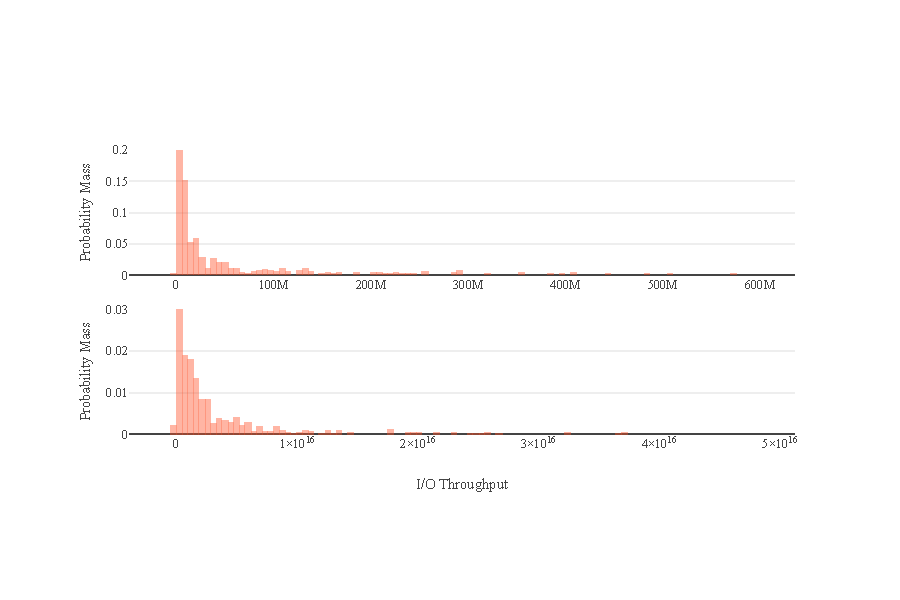
\includegraphics[width=\textwidth,trim={0 .5in 0 .4in}]{Raw_Throughput.pdf}
  \caption{Histograms of 100-bin reductions of the PMF of I/O
    throughput mean (top) and I/O throughput sample variance
    (bottom). In the mean plot, the first 1\% bin (truncated in plot)
    has a probability mass of .45. In the variance plot, the first 1\%
    bin has a probability mass of .58. It can be seen that the
    distributions of throughputs are primarily of lower magnitude with
    occasional extreme outliers.}
  \label{fig:raw_throughput}
\end{figure}

\subsection{Dimensional Analysis}
This work utilizes an extension to standard $k$-fold cross validation
that allows for a more thorough investigation of the expected model
performance in a variety of real-world situations. Alongside
randomized splits, two extra components are considered: the amount of
training data provided, and the dimension of the input data. It is
important to consider that algorithms that perform well with less
training input also require less experimentation. Although, the amount
of training data required may change as a function of the number of
input dimensions and this needs to be studied as well. The framework
used here will be referred to as a multidimensional analysis (MDA) of
the IOzone data.

%% \color{red}

\subsubsection{Multidimensional Analysis}
This procedure combines random selection of training and testing
splits with changes in the input dimension and the ratio of training
size to testing size. Given an input data matrix with $n$ rows
(points) and $d$ columns (components), MDA proceeds as follows:
\begin{enumerate}
\item for all $k = 1, \ldots, d$ and for all subsets of input
  components $F = \{ j_1, j_2, \ldots j_k \}$; reduce the input data
  to unique points $z \in \mathbb{R}^k$ with $f(z) = E[ \{ f(x^{(i)})
    \quad \forall i \quad s.t. \quad (x^{(i)}_F = z) \} ]$ where
  $x^{(i)}_F$ is the $k$-tuple containing only those components of
  $x^{(i)}$ in $F$.
\item for all $r$ in $\{5, 10, \ldots, 95\}$; generate $N$ random
  splits $(train, test)$ of the reduced data with $r$ percentage for
  training and $100 - r$ percentage for testing.
\item when generating each random $(train, test)$ split, ensure that
  all points from $test$ are on or inside the convex hull of points in
  $train$; also ensure that the points in $train$ are well spaced.
\end{enumerate}

In order to ensure that the testing points are inside the convex hull
of training points, this paper identifies the set of (reduced
dimension) points that compose the convex hull and forcibly places
those points in the training set. In order to ensure that training
points are well spaced, this paper relies on the statistical method
for picking points from \shortciteN{amos2014algorithm} that proceeds
as follows:
\begin{enumerate}
\item Generate a sequence of all pairs of points sorted by ascending
  pairwise $L_2$ distance between points, ${(x^{(i_1)},x^{(j_1)}),
    (x^{(i_2)},x^{(j_2)}), \ldots}$ such that
  $||x^{(i_k)}-x^{(j_k)}||_2 \leq ||x^{(i_{k+1})}-x^{(j_{k+1})}||_2$
\item Sequentially remove points from candidacy until only $N$ remain
  by randomly selecting one point from the pair $(x^{(i_k)},
  x^{(j_k)})$ for $k = 1,\ldots$ if both $x^{(i_k)}$ and $x^{(j_k)}$
  are still candidates.
\end{enumerate}

Given the large number of constraints, level of reduction, and use of
randomness in the MDA procedure, occasionally $N$ unique training
testing splits may not be created or may not exist. In these cases, if
there are fewer than $N$ possible splits then deterministically
generated splits are used. Otherwise after $3*N$ attempts, only the
unique splits are kept for analysis. The MDA procedure has been
implemented in python3 while most regression and interpolation methods
are FORTRAN wrapped with python. All randomness has been seeded for
repeatability.

For any input component subset $F$ (of size $k$) and selected value of
$r$, MDA will generate up to $N$ predictions that each multivariate
model has made for each point $z^{(i)} \in \mathbb{R}^k$. There may be
fewer than $N$ predictions made for any given point. Points in the
convex hull for the selected subset of components will always be used
for training, never for testing. Points that do not have any close
neighbors will often be used for training in order to ensure well
spacedness. Finally, as mentioned before, some subsets of components
do not readily generate $N$ unique training and testing splits.

MDA results in a distribution of possible estimates that a given
multivariate model could make for a point in $\mathbb{R}^k$, $k \leq
d$ given component set $F$. The summary results presented in this work
use the expected value of the distributions at each point as the model
estimate for error analysis.

%% is open source, and is freely available at the url
%% \textit{https://github.com/tchlux/VarSys/HPC\_Paper/Code/multi\_dim\_analysis.py}

%% \begin{enumerate}
%% \item Cycling the categorical settings
%% \item Selecting subsets of 1,2,3 up to 4 dimensions
%% \item Cycling different training : testing ratios (5:95 $\rightarrow$ 95:5)
%% \item Generating 200 random training : testing splits
%% \item Ensuring the testing points are on/inside the convex hull of the training.
%% \item Ensuring the training points are well-spaced.
%% \end{enumerate}

%% \subsection{Prediction}
%% \begin{enumerate}
%% \item For each file generated from the dimensional analysis, train on
%%   the training data, evaluate at the testing data points
%% \end{enumerate}

%     Results     
%=================
\section{Results}
\label{sec:results}

A na\"{\i}ve multivariate prediction technique such as nearest
neighbor could experience relative errors in the range $[0,
  (\text{max}_f - \text{min}_f) / \text{min}_f ]$ when modeling a non
negative function $f$ from data. The IOzone mean data response values
span three orders of magnitude (as can be seen in Table
\ref{tab:data_type}) while variance data response values span six
orders of magnitude. It is expected therefore, that all studied
multivariate models perform better than a na\"{\i}ve approach,
achieving relative errors strictly less than $10^3$ for throughput
mean and $10^6$ for throughput sample variance. Ideally, models will
yield relative errors significantly smaller than 1.

\subsection{I/O Throughput Mean}

Almost all multivariate models analyzed make predictions with a
relative error less than 1 for most system configurations when
predicting the mean I/O throughput of a system given varying amounts
of training data. The overall best of the multivariate models,
Delaunay, consistently makes predictions with relative error less than
$.05$ (5\% error). In Figure \ref{fig:mean_tt_ratio} it can also be
seen that the Delaunay model consistently makes good predictions even
with as low as 5\% training data (43 of the 864 system configurations)
regardless of the dimension of the data.

\begin{figure}
  \centering
  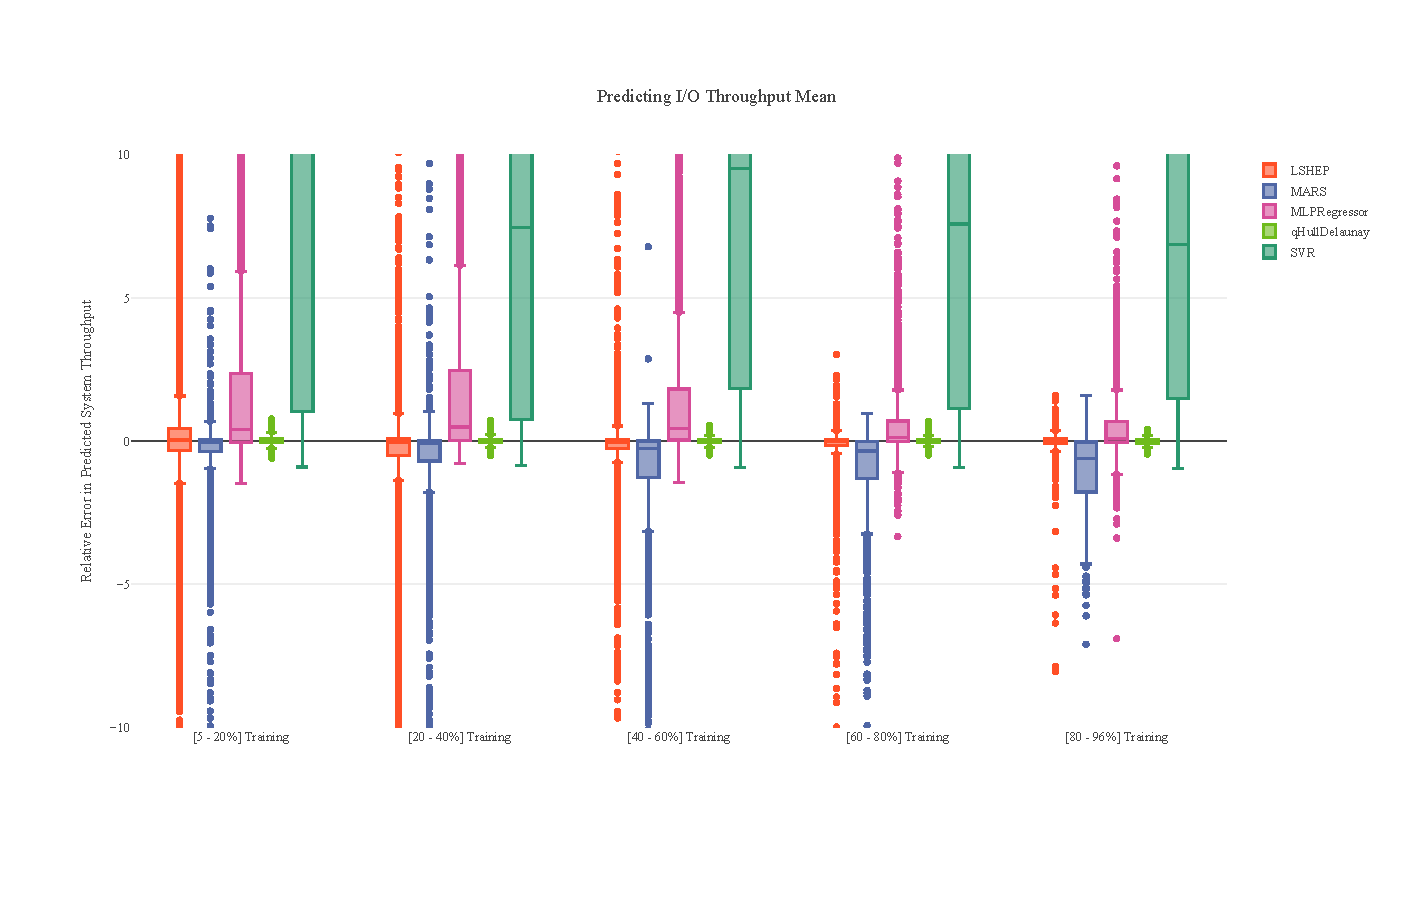
\includegraphics[width=\textwidth,trim={0 .5in 0 .5in}]{Mean_TT_Ratio.pdf}
  \caption{These box plots show the prediction error of mean with
    increasing amounts of training data provided to the models. Notice
    that MARS is the only model whose average spread of performance
    decreases with more training data. Recall that the response values
    being predicted span three orders of magnitude and hence relative
    errors should certainly remain within that range. For SVR the top
    box whisker goes from around 100 to 50 from left to right and is
    truncated in order to maintain focus on more performant models.}
  \label{fig:mean_tt_ratio}
\end{figure}

\begin{figure}
  \centering
  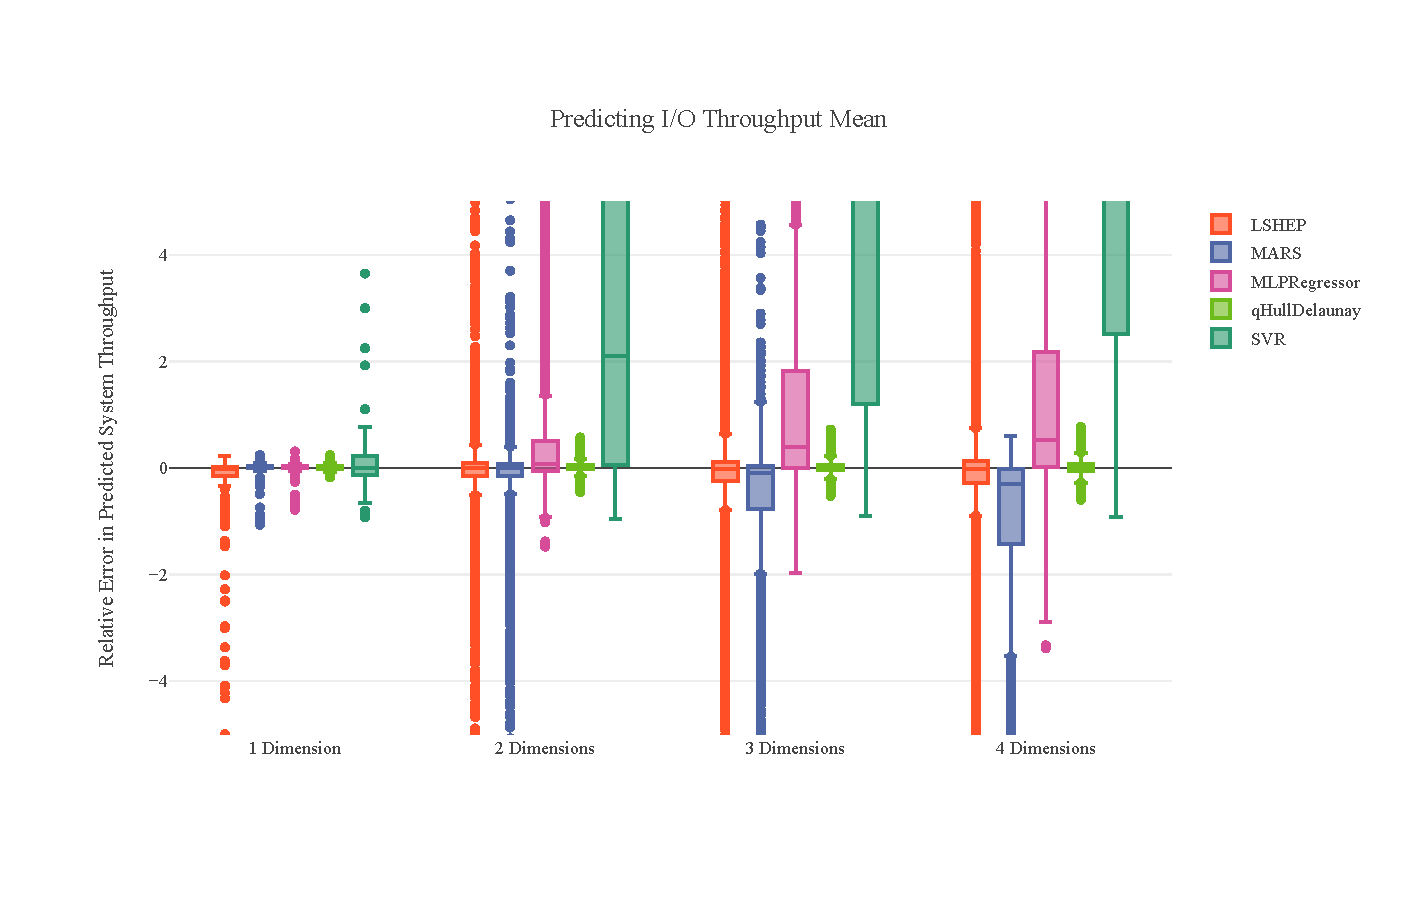
\includegraphics[width=\textwidth,trim={0 .5in 0 .5in}]{Mean_Dim.pdf}
  \caption{These box plots show the prediction error of mean with
    increasing dimension. The top box whisker for SVR transitions
    \{40, 80, 90\} for dimensions 2, 3, and 4 respectively. Notice
    that each model consistently experiences greater magnitude error
    with increasing dimension.}
  \label{fig:mean_dim}
\end{figure}

\subsection{I/O Throughput Variance}

The prediction results for variance resemble those for predicting
mean. Delaunay remains the best overall predictor with relative error
of .6 on average and LSHEP closely competes with Delaunay having an
average relative error of -2. Outliers in prediction error are much
larger for all models. Delaunay produces relative errors as large as
78 and other models achieve relative errors around $10^3$. The
relative errors for many models scaled proportional to the increased
orders of magnitude spanned by the variance response compared with
mean response. All models are more sensitive to the amount of training
data provided than their counterparts for predicting mean.

\subsection{Increasing Dimension and Decreasing Training Data}

As can be seen in Figure \ref{fig:mean_dim}, all of the models suffer
increasing error rates in higher dimension. This is expected, because
the number of possible interactions to model grows
exponentially. However, LSHEP and Delaunay maintain the slowest
increase in relative error. The increase in error seen for Delaunay
suggests that it is capable of making predictions with a range of
relative errors that grows approximately linearly with increasing
dimension input. This trend suggests that Delaunay would remain a
viable technique for accurately modeling systems with 10's of
parameters given only small amounts of training data. All models, with
the exception of MARS, produce smaller errors given more training
data. Increasing the amount of training data most notably reduces the
number of prediction error outliers.

%     Discussion     
%====================
\section{Discussion}
\label{sec:discussion}

The present results demonstrate that a straightforward application of
multivariate modeling techniques can be used to effectively predict
HPC system performance. Little effort on the part of a systems
engineer combined with a minimal amount experimentation can yield a
model capable of accurately tuning an HPC system to the desired
performance specification.

\subsection{Modeling the System}

The modeling techniques generated estimates of drastically different
quality when predicting I/O throughput mean and sample variance. A few
notable characteristics include: the SVR has the largest range of
errors for all selections of dimension and amount of training data;
MARS and LSHEP produce similar magnitude errors while the former
consistently underestimates and the latter consistently overestimates
in predictions; and Delaunay has considerably fewer outliers than all
other methods. SVR likely experiences the greatest quantity of errors
because the underlying parametric representation is global and
oversimplified (a single polynomial), making it unable to capture the
complex local behaviors of system I/O. It is still unclear however
what causes the behaviors of LSHEP, MARS, and Delaunay. An exploration
of this topic is left to future work.

While the Delaunay method appears to be the best predictor in the
presented IOzone case study, it is important to note its significantly
higher computational complexity with respect to the dimension of the
input. The implementation of Delaunay used would experience
unacceptably large training times beyond seven dimensions of
input. This leaves much room for other techniques to perform best in
higher dimension unless a more performant implementation of Delaunay
can be used.

Finally, the ability of the models to predict variance was
significantly worse for I/O sample variance. The larger scale in
variance responses alone do not account for the increase in relative
errors witnessed. This suggests that system variability has an greater
underlying functional complexity when compared with the system mean
and that latent factors are reducing prediction performance
considerably.

\subsection{Extending the Analysis}

System I/O throughput mean and throughput sample variance are simple
and useful system characteristics to model. The process presented in
this work is equally applicable to predicting other useful performance
characteristics of HPC systems such as: computational throughput,
power consumption, processor idle time, context switches, RAM usage,
or any other ordinal performance metric. For each of these there is
the potential to model system variability as well. This work has
chosen variance as a measure of variability, but the techniques used
in this paper could be used to predict more precise measures of
variability such as the percentiles of the performance distribution. A
thorough exploration of HPC systems applications of multivariate
modeling is left to future work.

%% \begin{enumerate}
%% \item Measuring different system characteristics other than I/O
%% \item Recording system performance constantly to maintain model accuracy
%% \end{enumerate}

\section{Conclusion}
\label{sec:conclusion}
Multivariate models of HPC systems produce promising results when
applied to predicting I/O throughput mean and variability. These
multivariate techniques significantly expand the comprehensiveness and
portability of statistical models for predicting computer system
performance over previous works. In the IOzone case study presented,
the Delaunay method produces the best overall results making
predictions for 821 system configurations with less than 5\% error
when trained on only 43 configurations. Analysis also suggests that
the error in the Delaunay method will remain manageable as the number
of system parameters being modeled increases. These multivariate
techniques can and should be applied to HPC systems with more than
four tunable parameters in order to identify optimal system
configurations that may not be discoverable via previous methods nor
by manual performance tuning.

%     Future Work     
%=====================
\subsection{Future Work}
The most severe limitation to the present work is the restriction to
modeling strictly ordinal (not categorical) system parameters. This
could be seen as a limitation of the multivariate models selected,
because only MARS is capable of handling non numeric components, or as
a limitation of the MDA framework. Future work could attempt to
identify the viability of different techniques for making predictions
across varying categorical system paramters.

There remain many other multivariate modeling techniques not included
in this work that should be evaluated and applied to HPC performance
tuning. For I/O alone, there are far more than the four tunable
parameters studied in this work. Alongside experimentation with more
models, there is room for a theoretical characterisation of the
combined model and data properties that allow for the greatest
predictive power.

%% \color{black}

%% \newpage
%% \ \\

%% \vspace{3in}

%% \texttt{\textbf{L}oc\textbf{A}ll\textbf{Y} li\textbf{NE}ar
%%   \textbf{W}eighted \textbf{A}pproxima\textbf{T}ion\textbf{S}
%%   \textbf{O}f fu\textbf{N}tions}\\
%% %% \texttt{L\ \ A\ \ Y \ \ NE\ \ \  W\ \ \ \ \ \ \ \ A\ \ \ \ \ \ \ \ T\ \ \ S O\ \ \ \ N\ \ \ \ \ \ }
%% \newpage

\bibliographystyle{scsproc}
\bibliography{paper}

\end{document}
